\documentclass{article}
\newcommand{\Nif}{$^{56}$Ni }
\usepackage{graphicx}
\begin{document}
\title{fast declining, low luminosity type Ia supernovae}
\maketitle

\section{\Nif mass}
We infer the $M_{^{56}Ni}$ for the low-luminosity SNe. For 91bg-like objects we find that the objects produce $\leq$ 0.1 $M_{\odot}$

The $M_{^{56}Ni}$ is computed from the bolometric maximum using Arnett's rule with a fixed rise time, as described in Stritzinger+2006. The bolometric light curves were corrected for host galaxy dust extinction using a cardelli law with $R_V$=3.1

\begin{table}
\begin{tabular}{ccccc}

\hline
SN & $M_{Ni}$ & Error & $s_{BV}$ & Classification \\
\hline
SN2006mr & 0.05 & 0.013 & 0.260 & 91bg \\
SN2007ax & 0.08 & 0.025 & 0.360 & 91bg \\
SN2007N & 0.07 & 0.011 & 0.297 & 91bg \\
SN2009F & 0.10 & 0.015 & 0.335 & 91bg \\
SN2005ke & 0.13 & 0.04 & 0.419 & 91bg \\
SN2007on & 0.30 & 0.09 & 0.574 & 86G \\
SN2008R & 0.26 & 0.06 & 0.594 & 86G \\
SN2007ba & 0.35 & 0.04 & 0.547 & ? \\
SN2005bl & 0.10 & 0.04 & 0.394 & 91bg \\
SN2007mm & 0.13 & 0.04 & 0.500 & 91bg \\
\hline
\end{tabular}
\caption{Nickel mass values for 91bg-like and 86G-like objects}
\end{table}


\begin{figure}
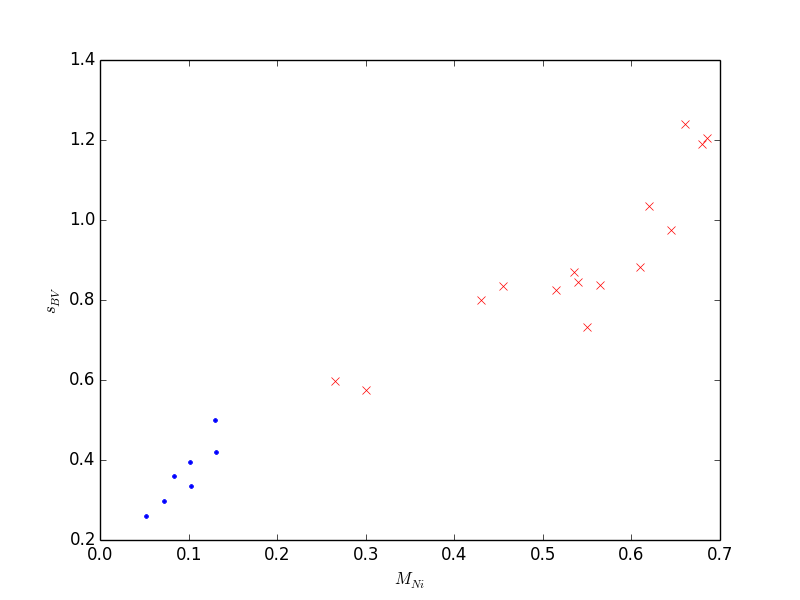
\includegraphics[width=0.7\textwidth]{../../diag_plots/sbv_mni_fast_norm.png}
\caption{'colour stretch' parameter plotted against the inferred $M_{^{56}Ni}$. \emph{Red}: Normal Ia's in the low-reddening sample. \emph{Blue}: Fast decliners}
\end{figure}

\section{NIR properties}
In this section, we look at the properties of fast declining objects in the NIR. The Near Infrared provides useful information to distinguish fast, faint SN~Ia from the normal  population, for e.g. normal Ia's show the NIR peak 2-6\,d \emph{before} B-band maximum light and show a prominent second peak in the $iYJHK$ bands.

\subsection{NIR primary maximum}
For our sample, we analyse the NIR primary maximum for the objects of interest. 
2007ba:
The $Y$ band has a first peak almost contemporaneous with $B$-max while the $J$ band is $\sim$ 1\,d later. The $H$ band peak is $\sim$ 1\,d \emph{earlier} than the $B$-max. 










\subsection{Objects with second maximum}
Sn~1991bg-like objects do not have enough line-blanketing opacity for the creation of two distinct maxima and hence show the appearance of a single 'late' second maximum which appears a few days post $B_{max}$. However, in a few cases, underlumnious Ia's have shown weak second maximum-like features in the NIR light curves

1. SN2003gs: A known fast decliner with multi-band photometry and spectral time series, 03gs, shows a prominent TiII trough in its near maximum spectra. with a $\Delta m_{15}$ of $\sim$ 1.83, it is a very fast declining Ia and has been classified as a 91bg-like. 
However, in its $J$ band light curve, there is a distinct appearance of a second maximum, at +15 days, which is earlier than the average of $\sim$ 28 days. This is not observed in objects with a similar decline rate, eg. SN2006mr. From the reddening corrected bolometric light curve, the total $M_{Ni}$ for the SN is 0.1 $M_{sun}$

2. SN2005ke:
The near maximum spectra show a TiII trough, but there is an appearance of a secondary bump-like feature at $\sim$ +15 days. SN2005ke has late time spectra available at $\sim$ +150 days 


3. SN2007ba: 
In Stritzinger+2011 (CSP2 data release) 2007ba has been classified as a 91bg-like. The near maximum spectra do show the TiII trough, but its less prominent compared to other faint objects. 
The $\Delta m_{15}$ value is 1.65 and the computed $M_{^{56}Ni}$ is 0.35  $M_{\odot}$. This suggests a greater production of Nickel than is expected for a 91bg-like.
The SN also shows a second maximum in the $Y$ and $i$ bands at $\sim$ +20 days. 

\subsection{Peak Width- Decline rate}
Faint and fast declining SNIa's are seen to exhibit only a single maximum in the NIR, which occurs a few days after the maximum in the optical. In Krisciunas et al. [2009], the single maximum was posited as a merger of the two maxima since the second maximum becomes progressively earlier for fainter objects. This would imply that the width of the single peak in 91bg-like SNe is correlated with the intrinsic brightness and hence, the decline rate. 
We measure the peak width as the time between the SN being 0.5 mag fainter before maximum and 0.5 mag fainter after maximum. We plot this value of the width against the 'colour stretch' parameter from Burns+ 2014. 

\begin{figure}
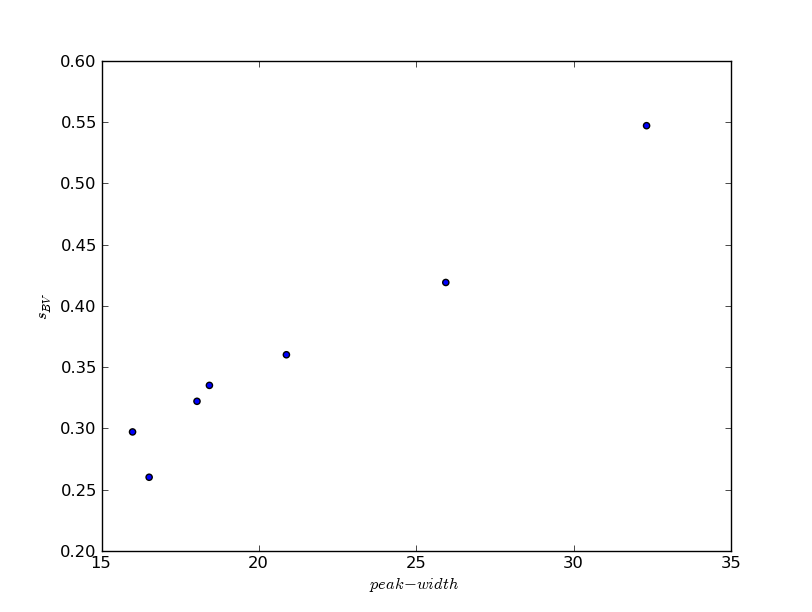
\includegraphics[width=.6 \textwidth]{../img/peak-width_sbv.png}
\caption{$s_{BV}$ is plotted against the width of the peak in the $Y$ band for 7 SNe which have sufficient early and late time data}
\end{figure}

We find that for the sample of 7 SNe, the peak-width in the $Y$ band is correlated with the $s_{BV}$ parameter, indicating that objects with wider light curves are brighter. 

\section{Spectral Properties}
In Nugent et al. [1995], the authors found a strong correlation between the peak B-band luminosity and the flux ratio between the Si II 5972 and Si II 6355 lines. This was msotly driven by the different line strengths of Si II 5972, arising from a variation in total IME's (with less luminous SNe having a greater value of this ratio). On similar lines, Hachinger et al. [???] showed that the equivalent widths of the Si II 5972 lines and Si II 4130 lines were strongly correlated with the decline rate parameters, proving that this line is a good indicator of intrinsic brightness. 

However, this relation is true for samples with 'normal' SNIa. For fast decliners, we find that there is almost no trend between the Si II width and the $\Delta m_{15}$. 
\subsection{Si II 4130}
\begin{figure}
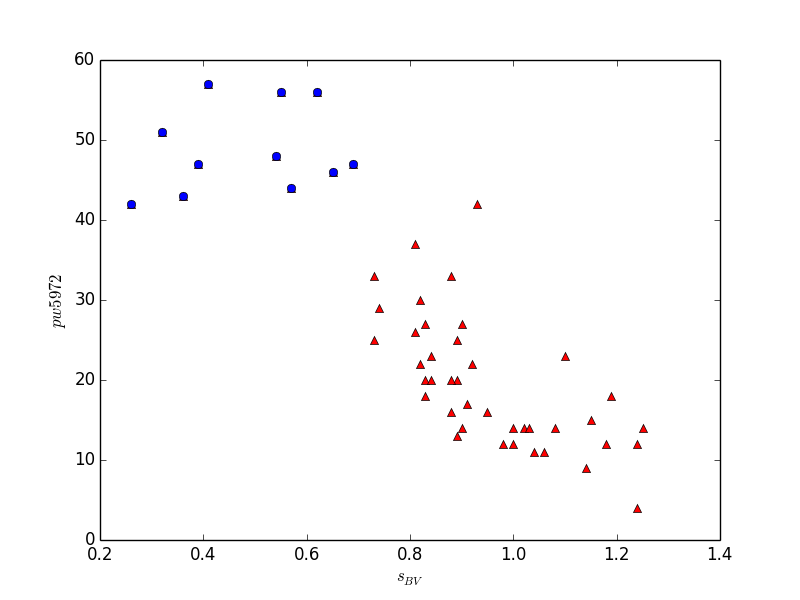
\includegraphics[width=.7\textwidth, trim= 0 30 0 30]{../img/pw5972_sbv.png}
\caption{The pseudo-equivalent width of SI II 5972 plotted against $s_{BV}$. blue points are objects with $s_{BV}$ < 0.7 roughly corresponding to the fast decliners with $\Delta m_{15}$ < 1.5. }
\end{figure} 

\subsection{SIIW }
For the complete sample of Ia's there is only a weak correlation ($r \sim$ 0.45) between the pseudo-equivalent width of the SIIW feature and $s_{BV}$. No such trend is seen with $\Delta m_{15}$.

For low luminosity events (defined by $s_{BV}$ < 0.7 or $\Delta m_{15}$ > 1.5) this trend is much stronger ($r \sim$ 0.9). 

\begin{figure}
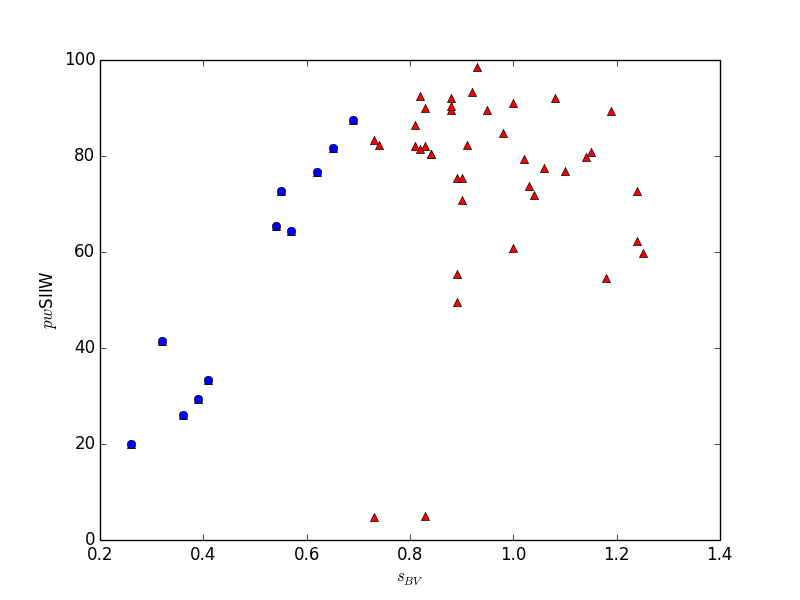
\includegraphics[width=.7\textwidth, trim= 0 30 0 30]{../img/pwSIIw_sbv.png}
\caption{The pseudo-equivalent width of SIIW plotted against $s_{BV}$. blue points are objects with $s_{BV} <$ 0.7 roughly corresponding to the fast decliners with $\Delta m_{15}$ $>$ 1.5. }
\end{figure} 


\subsection{Fe II line $\sim$ + 20\,d}

\end{document}
